\chapter{Kort}
\label{kort}

\begin{center}
\begin{figure}[H]
\begin{center}
\subfigure{
\includegraphics[scale=0.8]{images/implementation/frontend/kort-icon_with_gloss}}
\hspace{1cm}
\subfigure{
\includegraphics[scale=0.8]{images/implementation/frontend/kort_herokuapp_com-qrcode}}
\end{center}
\end{figure}

{\Large \textbf{\url{http://kort.herokuapp.com/}}}

\vspace{1cm}

\begin{figure}[H]
\subfigure{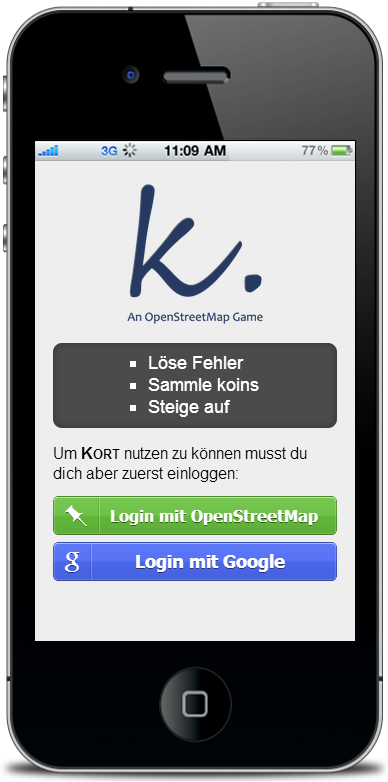
\includegraphics[width=0.3\textwidth]{images/screenshots/kort-screenshot-login}}
\hfill
\subfigure{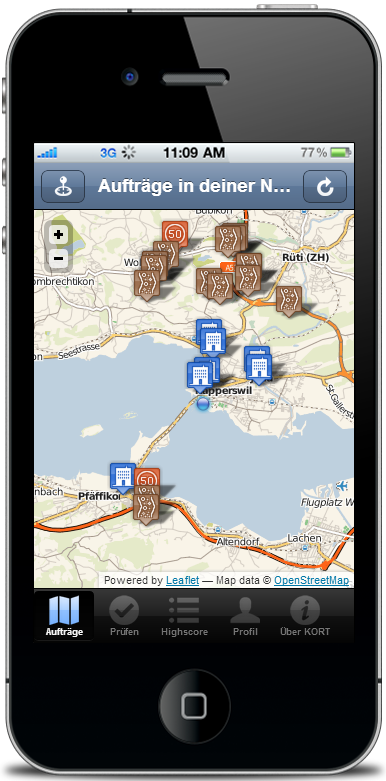
\includegraphics[width=0.3\textwidth]{images/screenshots/kort-screenshot-bugmap}}
\hfill
\subfigure{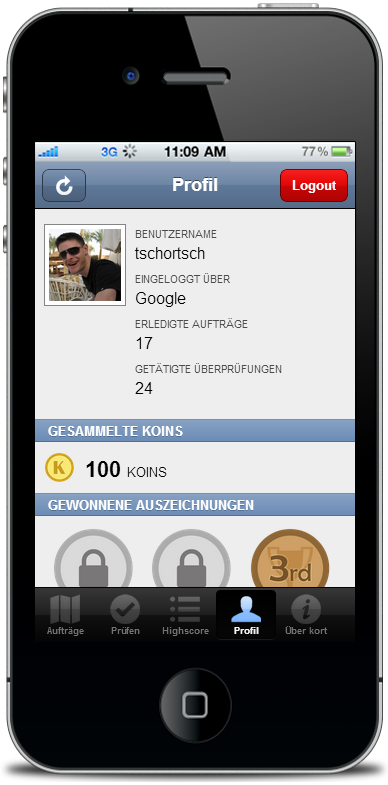
\includegraphics[width=0.3\textwidth]{images/screenshots/kort-screenshot-profile}}
\end{figure}
\end{center}

% Analyse
% Analyse
\section{Analyse}

% User Szenarien
\subsection{User Szenarien}
\label{kort-user-szenarien}

Um die Anforderungen an die App genauer abschätzen zu können, wurden im Vorfeld der Implementierung einige Szenarien erstellt.

\subsubsection{Szenario 1: Zeitvertreib an der Bushaltestelle}

Simon muss 15 Minuten an der Bushaltestelle auf den nächsten Bus warten.
Um sich die Wartezeit zu verkürzen, nimmt er sein Smartphone hervor und startet die \kort{}-Applikation.

Die App hat ihn bereits lokalisiert und zeigt ihm offene \brand{OpenStreetMap}-Aufträge in der Nähe, wahlweise als Liste oder auf der Karte an.
Für die Aufträge werden Simon verschiedene Belohnungen angeboten, abhängig vom Schwierigkeitsgrad der Aufgabe.

Simon entscheidet sich für einen Auftrag mit mittlerer Belohnung.
Die App zeigt ihm den Weg zum Auftrag und erklärt, was zu tun ist.
Beim Auftrag handelt es sich um einen fehlenden Strassennamen.

Als Simon vor Ort ist, findet er sehr schnell ein Strassenschild.
Er gibt den Namen in der App ein wofür er bereits 10 Punkte erhält.
Da er zusätzlich sogar noch ein Foto hochlädt, bekommt er weitere 5 Punkte.

Der Auftrag ist somit für ihn erledigt, was ihm entsprechend von der App mitgeteilt wird.
Danach verschwindet der Auftrag aus seiner Auftragsliste und von der Karte.

\textbf{Ziele}
\begin{itemize}
\item Zeitvertreib
\item Punkte sammeln
\item Daten verbessern
\end{itemize}

\subsubsection{Szenario 2: Validieren}

Andy sitzt im Zug und langweilt sich.
Er öffnet die \kort{}-App im Indoor-Modus und sieht sich die Liste der zu validierenden Lösungsvorschläge an. 
Er sortiert die Liste, um diejenigen Einträge zu sehen, welche nur noch einen Review benötigen, um an \brand{OpenStreetMap} gesendet werden zu können.

Er öffnet einen Vorschlag für einen fehlenden Strassennamen in der Umgebung.
Er kennt zwar die Gegend ist sich aber nicht 100\% sicher ob der Name stimmt.
Um sicherzugehen, öffnet er das angehängte Bild.
Das Bild zeigt ein Strassenschild, welches mit dem eingegeben Namen übereinstimmt
Andy bestätigt dann die Änderung und schliesst den Bug damit ab.

\cleardoublepage
\textbf{Ziele}
\begin{itemize}
\item Schnell und einfach geeignete Einträge zum Validieren finden
\item Qualität der Änderungen sicherstellen
\end{itemize}

\subsubsection{Szenario 3: Erster Kontakt zur App}

Über den Kurznachrichtendienst Twitter sieht Monika, dass ihre Kollegin gerade das erste mal \kort{} gestartet hat.
Als sie auf den Link klickt öffnet sich ihr Browser und die App wird angezeigt.
Da es sich um ihren ersten Besuch auf der Seite handelt, wird ihr kurz erklärt um was es geht.

Danach sieht sie die Karte mit den vorhandenen Fehlereinträgen.
Bevor sie einen Eintrag bearbeiten kann, muss sie sich anmelden.
Sie wählt dazu einen Benutzernamen und wird anschliessend auf die Seite von Google weitergeleitet, um sich anzumelden.
Nach dem erfolgreichen Login wird Monika zurück zur \kort{}-App geleitet, wo sie beginnen kann, die ersten Aufträge zu erfüllen.

\textbf{Ziele}
\begin{itemize}
\item Direkt ersichtlich, was die App kann
\item Schneller Einstieg
\item Einfache Anmeldung (keine Registrierung!)
\item Benutzerführung durch die Funktionen
\end{itemize}

\subsubsection{Szenario 4: Highscore-Anwärter}

Edi benutzt schon seit einiger Zeit die \kort{}-App und hat in seinem Revier bereits den zweiten Platz der Highscore erreicht.
Seine Platzierung überprüft er regelmässig in der App.

Heute möchte er endlich die Spitze erklimmen und den "`Leader"'-Badge erhalten.
Dazu hat er sich einige Aufträge ausgesucht, welche er der Reihe nach bearbeiten will.
Bei jedem Auftrag sieht Edi, wie viele Punkte er sammeln kann.

Nachdem er den 5. Auftrag erfolgreich erledigt hat, erhält er eine Benachrichtigung, dass er den "`Leader"'-Badge erhalten hat.
Auch in der Rangliste steht Edi nun zuoberst.

\textbf{Ziele}
\begin{itemize}
\item Einfach mehrere Aufträge nacheinander ausführen
\item Badges sammeln
\item Highscore anzeigen
\item Erster Rang erreichen
\end{itemize}

% Paper-Prototype
\subsection{Paper-Prototype}
% Subfigure counter zuruecksetzen
\setcounter{subfigure}{0}

Aus den gesetzten Projektzielen und den Anforderungen der erstellten Szenarien (siehe Abschnitt \ref{kort-user-szenarien}) wurde vor der Implementation der Oberfläche ein Paper-Prototype des GUI-Designs erstellt.
Der Prototype besteht aus vier Hauptmasken und einem Overlay für den Login.

\subsubsection{Overlay: Login}
Beim ersten Starten der \gls{WebApp} erhält man die Möglichkeit sich über verschiedene Dienste anzumelden.
Mit einem Klick auf den jeweiligen Anbieter, wird man zu diesem weitergeleitet und kann sich dort anmelden.

\begin{figure}[H]
\subfigure[Login - Anbieterauswahl]{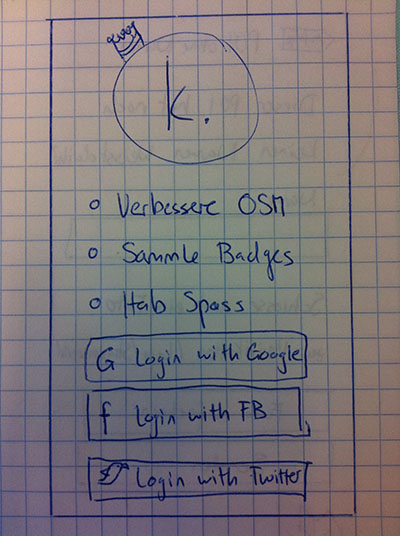
\includegraphics[width=0.43\textwidth]{images/paperprototype/kort-pp-startscreen}}
\hfill
\subfigure[Login - Loginformular des jeweiligen Anbieters]{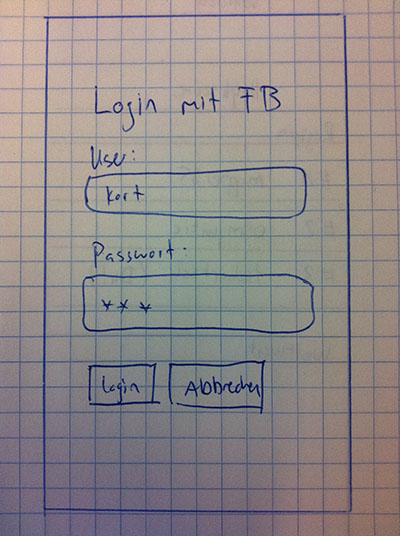
\includegraphics[width=0.43\textwidth]{images/paperprototype/kort-pp-login}}
\end{figure}

\cleardoublepage
\subsubsection{Maske: Aufträge}
Nachdem sich der Benutzer erfolgreich angemeldet hat, erscheint die Maske mit den Aufträgen.
Darauf werden die vorhandenen Fehler auf einer Karte angezeigt.
Es werden jeweils nur die Fehler angezeigt, welche sich in unmittelbarer Nähe des eigenen Standorts befinden.
Die Fehler werden mit einer Markierung auf der Karte dargestellt.

Durch Anklicken einer solchen Markierung öffnet sich die Detailansicht des Fehlers, wo sich der Fehler direkt beheben lässt.
Neben der Möglichkeit, einen Lösungstext einzugeben, soll es auch möglich sein, ein Beweis-Foto hochzuladen.
Mit einem Klick auf den Senden-Knopf schliesst sich die Detailansicht und man gelangt zur Karte mit den Aufträgen zurück.

\begin{figure}[H]
\subfigure[Aufträge - Karte mit Fehlern]{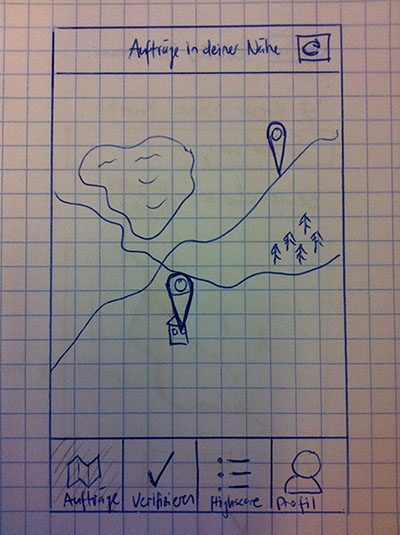
\includegraphics[width=0.43\textwidth]{images/paperprototype/kort-pp-bugs}}
\hfill
\subfigure[Aufträge - Detailansicht eines Fehlers]{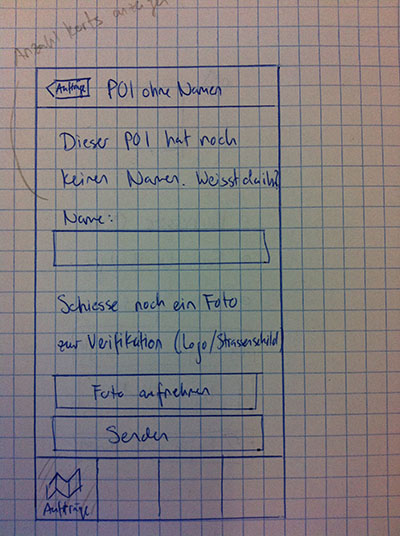
\includegraphics[width=0.43\textwidth]{images/paperprototype/kort-pp-fix}}
\end{figure}

\cleardoublepage
\subsubsection{Maske: Verifizieren}
Auf der Verifikationsmaske werden die bereits gelösten Fehler in der Nähe angezeigt.
Sie sind gruppiert nach Anzahl nötigen Verifikationen, um sie an \brand{OpenStreetMap} zurückzusenden.

Per Klick auf einen Eintrag öffnet sich die Verifikationsmaske.
Darin wird der Fehlerlösungstext und das Beweis-Foto angezeigt.
Zusätzlich wird das betroffene \brand{OpenStreetMap}-Objekt auf einer Karte angezeigt.
Man hat die Möglichkeit, die Problemlösung als \emph{Korrekt} oder \emph{Falsch} zu bewerten.

\begin{figure}[H]
\subfigure[Verifizieren - Liste mit Fehlerlösungen]{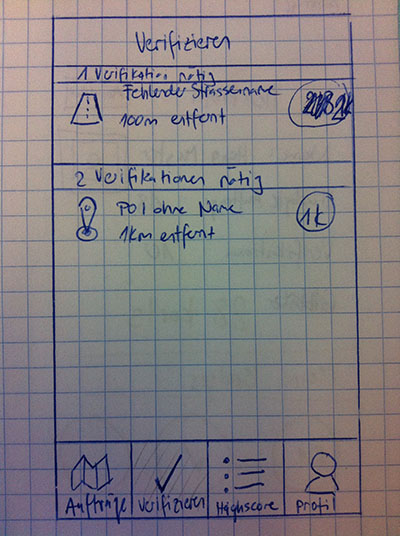
\includegraphics[width=0.43\textwidth]{images/paperprototype/kort-pp-verify}}
\hfill
\subfigure[Verifizieren - Detailansicht einer Fehlerlösung]{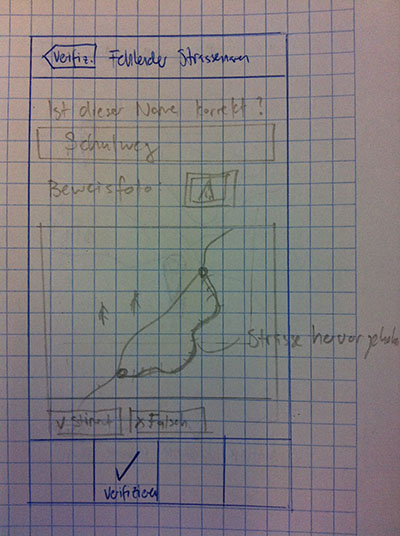
\includegraphics[width=0.43\textwidth]{images/paperprototype/kort-pp-verify_detail}}
\end{figure}

\cleardoublepage
\subsubsection{Maske: Highscore}
In der Highscore-Maske kann man sich mit anderen Spielern messen.
Man sieht seine eigene Platzierung und die der anderen Spieler.
Es werden Highscores für verschiedene Kategorien (z.B. regional, weltweit) angezeigt.

\subsubsection{Maske: Profil}
Im Profil werden die Eckdaten des eigenen Benutzers angezeigt.
Dazu gehören die Anzahl der gelösten Aufträge und die Anzahl der getätigten Verifikationen.
Zusätzlich werden die Gesamtanzahl der gesammelten Punkte und die gewonnenen Badges ausgewiesen.
Auf der Profil-Maske kann sich der Benutzer von der App abzumelden.

\begin{figure}[H]
\subfigure[Highscore]{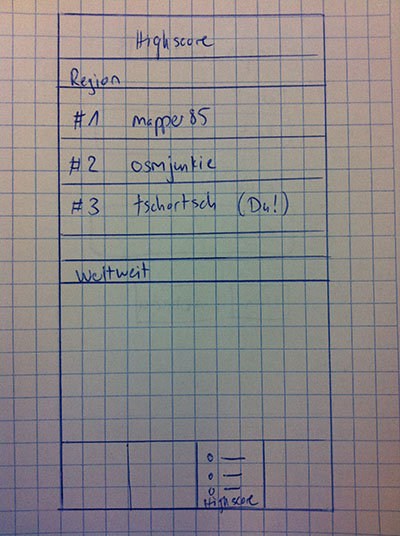
\includegraphics[width=0.43\textwidth]{images/paperprototype/kort-pp-highscore}}
\hfill
\subfigure[Profil]{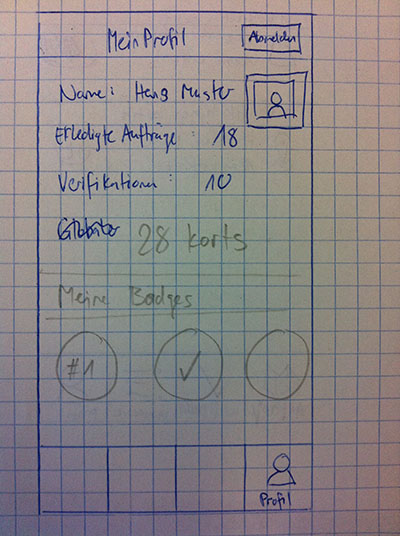
\includegraphics[width=0.43\textwidth]{images/paperprototype/kort-pp-profile}}
\end{figure}

% Design
% Design
\section{Design}

\subsection{Package-Struktur}

Die Package-Struktur wird vom \brand{Sencha Touch 2}-Framework vorgegeben. Sie entspricht grundsätzlich dem \gls{MVC}-Layout.
Speziell daran ist das Konzept der \emph{Stores}, welche einen beliebigen Datenspeicher abstrahieren.
Stores sind an ein \emph{Model} gebunden, welches die Struktur der gespeicherten Daten vorgibt.

Zusätzlich sind sie über einen \emph{Proxy} mit der Datenquelle verbunden.
Dabei kann es sich beispielsweise um einen \gls{REST}-Webservice handeln oder den \gls{Local Storage} des Browsers.

In Abbildung \ref{image-kort-packagediagram} wird die Package-Struktur von \kort{} mit deren Abhängigkeiten gezeigt.

\begin{figure}[H]
	\centering
	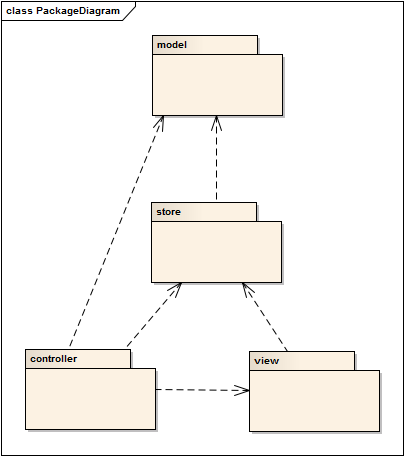
\includegraphics[scale=0.7]{images/uml/kort-packagediagram}
	\caption{Package-Struktur}
	\label{image-kort-packagediagram}
\end{figure}

\subsection{Controller-Package}

Die App ist so gestaltet, dass jede Hauptansicht einen eigenen Controller besitzt.
Dieser ist für die Steuerung der Benutzeroberfläche zuständig.

Die verschiedenen Controller lassen sich grob in drei Klassen einteilen.
Zunächst gibt es Controller für die einzelnen Masken der Applikation (siehe Abbildung \ref{image-kort-classdiagram-controller} $\rightarrow$ \emph{main tab controllers}).
Zusätzlich haben einige Tabs eine Detailansicht, welche ebenfalls von einem eigenen Controller gesteuert wird (siehe Abbildung \ref{image-kort-classdiagram-controller} $\rightarrow$ \emph{detail controllers}).
Zuletzt gibt es eigenständige Controller für die Overlay-Komponenten, welche die gesamte Oberfläche der App verdecken (siehe Abbildung \ref{image-kort-classdiagram-controller} $\rightarrow$ \emph{overlay controllers}).

\begin{figure}[H]
	\centering
	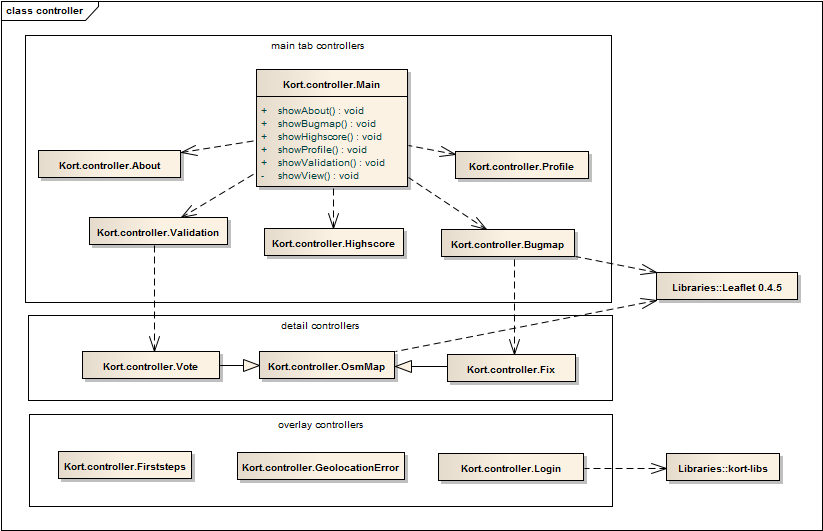
\includegraphics[width=\textwidth]{images/uml/kort-classdiagram-controller}
	\caption{Klassendiagramm der Controller}
	\label{image-kort-classdiagram-controller}
\end{figure}

\subsection{Store- und Model-Package}
\label{kort-store-model-package}

Die \emph{Stores} bilden die Datenspeicher in einer \brand{Sencha Touch} Applikation.
Über ein \emph{Model} wird die jeweilige Struktur der gespeicherten Daten festgelegt.
Stores sind zudem über einen \emph{Proxy} mit der Datenquelle verbunden.
Im Falle von \kort{} wurden dafür ausschliesslich \gls{REST}-Ressourcen verwendet (siehe Abbildung \ref{image-kort-classdiagram-store}).

\begin{figure}[H]
	\centering
	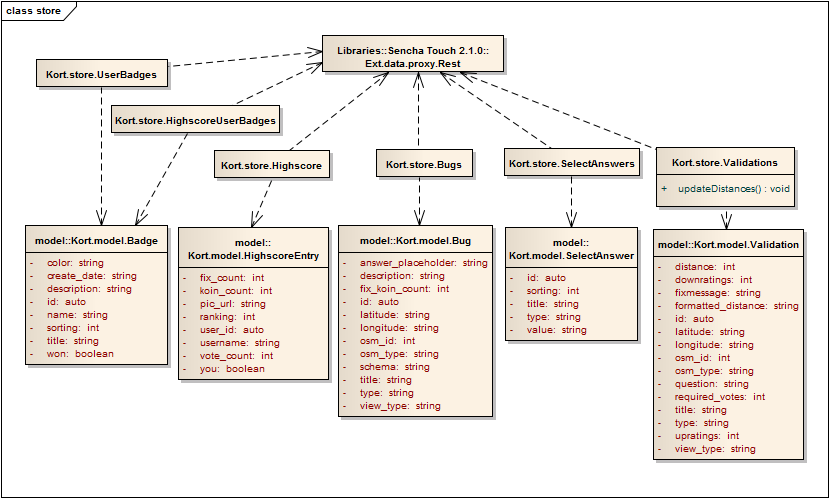
\includegraphics[width=\textwidth]{images/uml/kort-classdiagram-store}
	\caption{Klassendiagramm der Stores}
	\label{image-kort-classdiagram-store}
\end{figure}

\subsubsection{Models ohne Store}

Falls die Applikation jeweils nur eine Instanz eines \emph{Models} verwendet, können diese ohne einen Store direkt mit einem Proxy verbunden werden.
In \kort{} wurde dies für den eingeloggten Benutzer (User) sowie für die zu sendenden Datenpakete wie der Fehler-Lösung (Fix) und der Validierung (Vote) verwendet (siehe Abbildung \ref{image-kort-classdiagram-model_own_proxy}).

\begin{figure}[H]
	\centering
	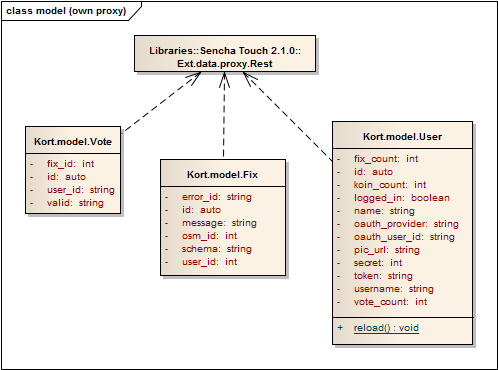
\includegraphics[scale=0.5]{images/uml/kort-classdiagram-model_own_proxy}
	\caption{Klassendiagramm der Models ohne Stores}
	\label{image-kort-classdiagram-model_own_proxy}
\end{figure}

\subsubsection{Speichern der Logininformationen}
Die Logininformationen des Benutzers werden im \gls{Local Storage} des Browsers abgelegt (siehe Abbildung \ref{image-kort-classdiagram-store_localstorage}).
Der genaue Ablauf wird in Abschnitt \ref{oauth} beschrieben.

\begin{figure}[H]
	\centering
	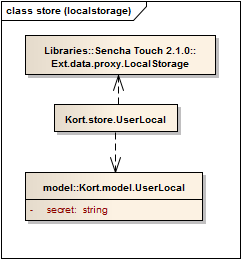
\includegraphics[scale=0.6]{images/uml/kort-classdiagram-store_localstorage}
	\caption{Speichern der Logininformationen im Local Storage}
	\label{image-kort-classdiagram-store_localstorage}
\end{figure}

\subsection{Aufbau der Benutzeroberfläche}
Jede Maske der Applikation befindet sich in einer eigenen View-Klasse.
Diese verschiedenen View-Klassen werden in der Hauptklasse \inlinecode{Kort.view.Main} inkludiert und angezeigt (siehe Abbildung \ref{image-kort-classdiagram-view}).

\begin{figure}[H]
	\centering
	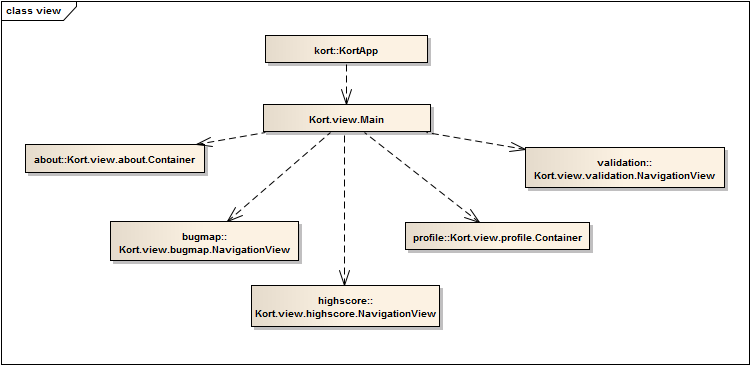
\includegraphics[width=\textwidth]{images/uml/kort-classdiagram-view}
	\caption{Aufbau der Benutzeroberfläche}
	\label{image-kort-classdiagram-view}
\end{figure}

% Implementation
\section{Implementation}
\label{backend-implementation}
Das Backend besteht neben der Datenbank und den \gls{REST}-Schnittstellen vor allem aus PHP-Code.
Der meiste Code entfällt auf das Handling von Webservice-Anfragen und die Authentifizierung mit \gls{OAuth}.

\subsection{Gliederung}
\label{backend-gliederung}
Das Backend befindet sich im Verzeichnis \inlinecode{server/} im Repository.
Das Backend teilt sich auf verschiedene Unterordner auf (siehe Tabelle \ref{table-backend-gliederung}).

\begin{table}[H]
\centering
\begin{tabular}{|p{0.25\twocelltabwidth}|p{0.75\twocelltabwidth}|}
\hline 
\textbf{Order} & \textbf{Inhalt} \\
\hline 
\inlinecode{database/} & SQL und Shell-Skripts für die Erstellung der Datenbank \\
\hline 
\inlinecode{heroku/} & Shell-Skripte für das Deployment auf Heroku \\
\hline 
\inlinecode{oauth2callback/} & Callback-Handler der verschiedenen \gls{OAuth}-Dienste \\
\hline 
\inlinecode{php/} & PHP-Klassen für das Backend \\
\hline 
\inlinecode{redmine/} & Skripts und Anleitung für Redmine \\
\hline 
\inlinecode{ssh\_pub\_keys/} & Öffentliche SSH-Schlüssel für das Deployment \\
\hline 
\inlinecode{webservices/} & \gls{REST}-Ressourcen (Endpunkte der Schnittstellen) \\
\hline 
\end{tabular}
\caption{Gliederung des Backends}
\label{table-backend-gliederung}
\end{table}

Speziell zu erwähnen sind dabei die PHP-Klassen, welche die Logik des Backends abbilden.
Sie sind über Namespaces aufgeteilt und liefern die Logik für alle anderen Teile des Backends.
Um dies zu ermöglichen, gibt es die \inlinecode{ClassLoader}-Klasse\footnote{\url{http://kort.herokuapp.com/docs/Kort-backend/classes/Kort.ClassLoader.html}}.
Falls irgendwo eine PHP-Klasse gebraucht wird, muss nur diese Klasse geladen werden, diese wiederum kümmert sich darum, alle abhängigen Dateien nachzuladen.

Für die Klassen gibt es eine separate Dokumentation (siehe Abschnitt \ref{backend-dokumentation}).

\subsection{Abhängigkeiten}
\label{backend-abhaengigkeiten}

\begin{table}[H]
\centering
\begin{tabular}{|p{0.35\threecelltabwidth}|p{0.15\threecelltabwidth}|p{0.50\threecelltabwidth}|}
\hline 
\textbf{Library} & \textbf{Version} & \textbf{Verwendung} \\
\hline 
Slim & 2.1.0 & Micro-Framework für die Implementation von \gls{REST}-Schnittstellen \\
\hline 
Google APIs Client Library & 0.6.0 & PHP-Library für Google \glspl{API} \\
\hline 
oauth-php & 175 & \gls{OAuth} Library für PHP \\
\hline 
Ant-Contrib & 1.0b3 & Erweiterte Tasks für Apache Ant \\
\hline 
\end{tabular}
\caption{Abhängigkeiten im Backend}
\label{table-backend-dependencies}
\end{table}



% Resultate
% Resultate
\section{Resultate}

\kort{} besteht aus fünf verschiedenen Hauptmasken.
Diese sind in der Applikation über die Tabs im unteren Bereich erreichbar.

\subsection{Maske: Aufträge}
In dieser Maske werden dem Benutzer alle noch nicht gelösten Fehler in seiner Umgebung als Markierungen auf der Karte angezeigt (siehe Abbildung \ref{maske-auftraege}).
Die Fehleranzahl ist dabei auf die 25 nächstgelegenen Fehler limitiert.

Beim Klick auf einen Fehler wird der Benutzer gefragt, ob er diesen auch wirklich lösen kann.
Bestätigt er, wird ihm der Fehler im Detail angezeigt.
In dieser Detailansicht wir ihm zudem je nach Fehlertyp ein Text- oder ein Auswahlfeld angezeigt, in welchem er die Antwort eingeben bzw. auswählen kann. 

Zusätzlich gibt es die Möglichkeit, sich den Fehler nochmals auf der Karte anzuzeigen zu lassen.
Dieser wird dabei als Geometrie-Objekt angezeigt.
Eine Strasse wird dabei beispielsweise als Linie oder ein Gelände als Polygon dargestellt.

\begin{figure}[H]
\subfigure{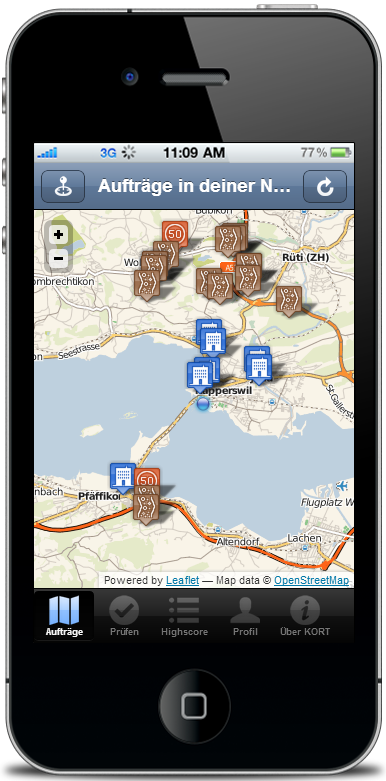
\includegraphics[width=0.3\textwidth]{images/screenshots/kort-screenshot-bugmap}}
\hfill
\subfigure{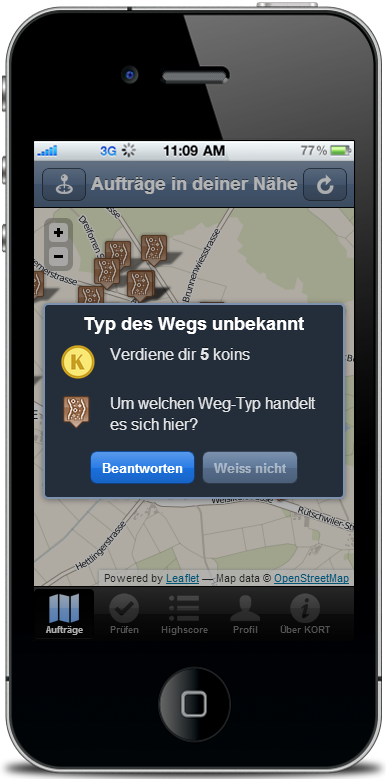
\includegraphics[width=0.3\textwidth]{images/screenshots/kort-screenshot-bugmap_message_box}}
\hfill
\subfigure{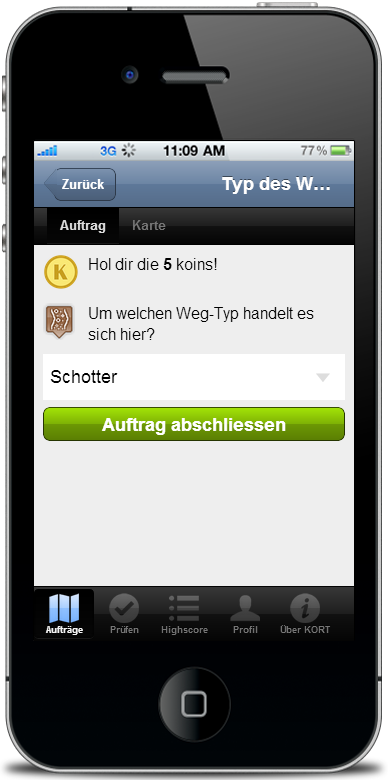
\includegraphics[width=0.3\textwidth]{images/screenshots/kort-screenshot-fix}}
\caption{Maske: Aufträge}
\label{maske-auftraege}
\end{figure}

\subsection{Maske: Prüfen}
In der \emph{Prüfen}-Maske werden dem Benutzer die Lösungen angezeigt, welche noch zu überprüfen sind (siehe Abbildung \ref{maske-pruefen}).
Diese sind dabei nach der Anzahl noch nötiger Überprüfungen gruppiert.
So soll erreicht werden, dass Lösungen, die schon bald an \brand{OpenStreetMap} zurückgesendet werden können, bevorzugt behandelt werden.
In der Liste werden maximal 25 Überprüfungen angezeigt.

Sobald der Benutzer einen Eintrag auswählt, wird ihm neben der eingetragenen Lösung auch der Fehler auf der Karte angezeigt.
Er kann nun beurteilen, ob diese Lösung korrekt oder falsch ist.

\begin{figure}[H]
\subfigure{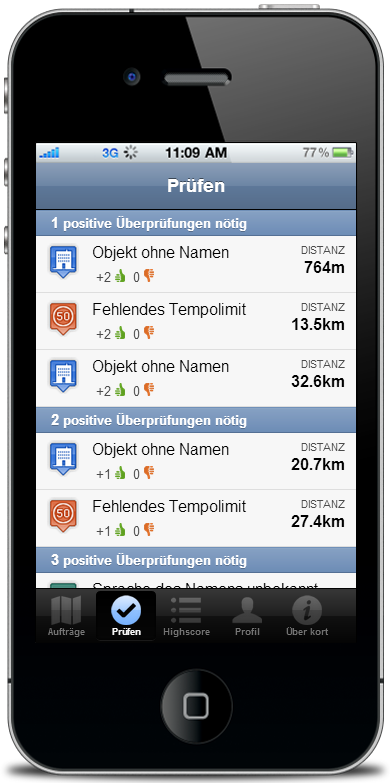
\includegraphics[width=0.3\textwidth]{images/screenshots/kort-screenshot-validation}}
\hfill
\subfigure{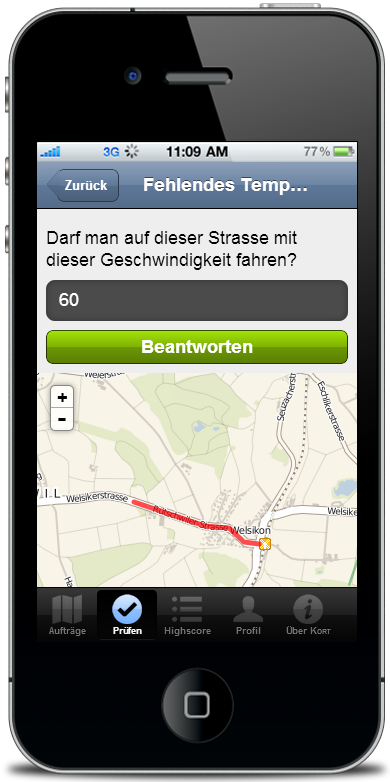
\includegraphics[width=0.3\textwidth]{images/screenshots/kort-screenshot-vote}}
\hfill
\subfigure{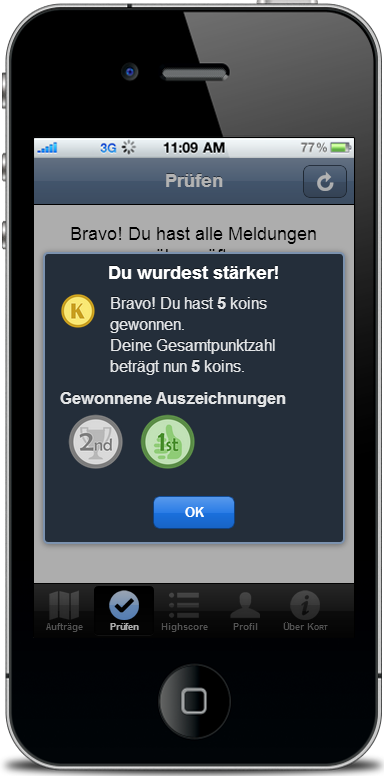
\includegraphics[width=0.3\textwidth]{images/screenshots/kort-screenshot-reward}}
\caption{Maske: Prüfen}
\label{maske-pruefen}
\end{figure}

\subsection{Maske: Highscore}
In der Highscore werden die Benutzer nach Anzahl gewonnener Punkte (sog. \emph{Koins}) sortiert (siehe Abbildung \ref{masken-highscore-profile-about}).
Es werden jeweils die ersten zehn Platzierungen angezeigt.

Wird ein Eintrag in der Highscore-Liste ausgewählt, so kann man sich das Profil des jeweiligen Benutzers anschauen.

\subsection{Maske: Profil}
Im Profil findet man eine Zusammenfassung seiner persönlichen Spielaktivitäten.
Man sieht die Gesamtanzahl der gesammelten \emph{Koins} und eine Übersicht der gewonnen Auszeichnungen (siehe Abbildung \ref{masken-highscore-profile-about}).

Auf der Profilseite lassen sich die Auszeichnungen auch in Grossformat anzeigen.

\subsection{Maske: Über Kort}
Auf der \emph{Über Kort}-Seite werden allgemeine Informationen zur Applikation angezeigt (siehe Abbildung \ref{masken-highscore-profile-about}).

\begin{figure}[H]
\subfigure{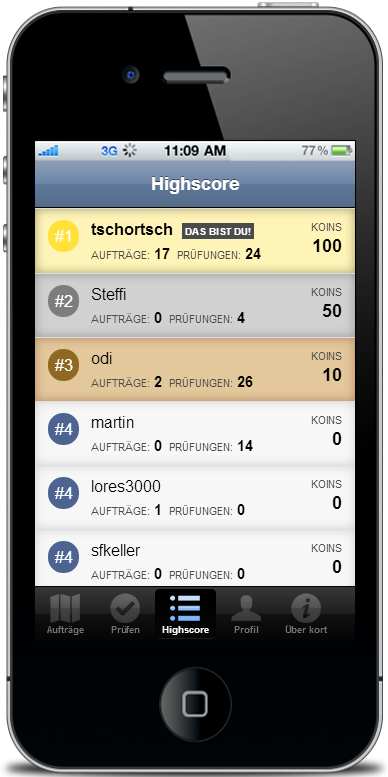
\includegraphics[width=0.3\textwidth]{images/screenshots/kort-screenshot-highscore}}
\hfill
\subfigure{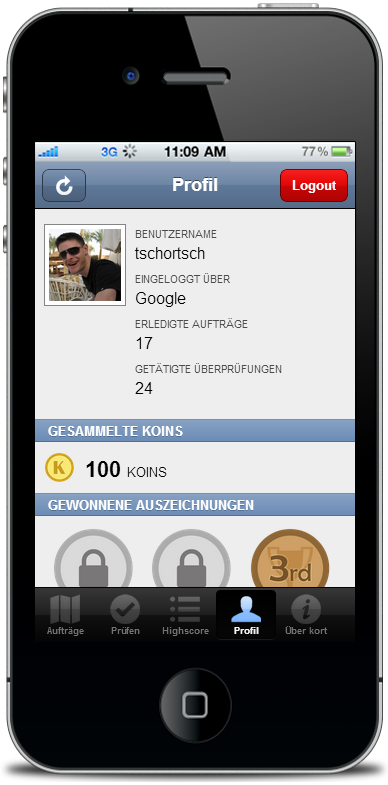
\includegraphics[width=0.3\textwidth]{images/screenshots/kort-screenshot-profile}}
\hfill
\subfigure{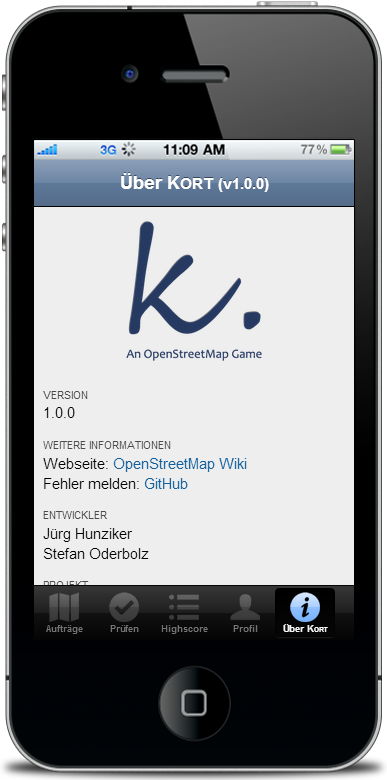
\includegraphics[width=0.3\textwidth]{images/screenshots/kort-screenshot-about}}
\caption{Masken: Highscore / Profil / Über \kort{}}
\label{masken-highscore-profile-about}
\end{figure}

% Dokumentation
% Dokumentation
\section{Dokumentation}

Das Frontend von \kort{} ist durchgängig mit der Sencha-eigenen Dokumentationssprache \brand{JSDuck}\footnote{\url{https://github.com/senchalabs/jsduck}} dokumentiert.
Die Dokumentation findet sich unter: \url{http://kort.herokuapp.com/docs/Kort}.

\begin{figure}[H]
	\centering
	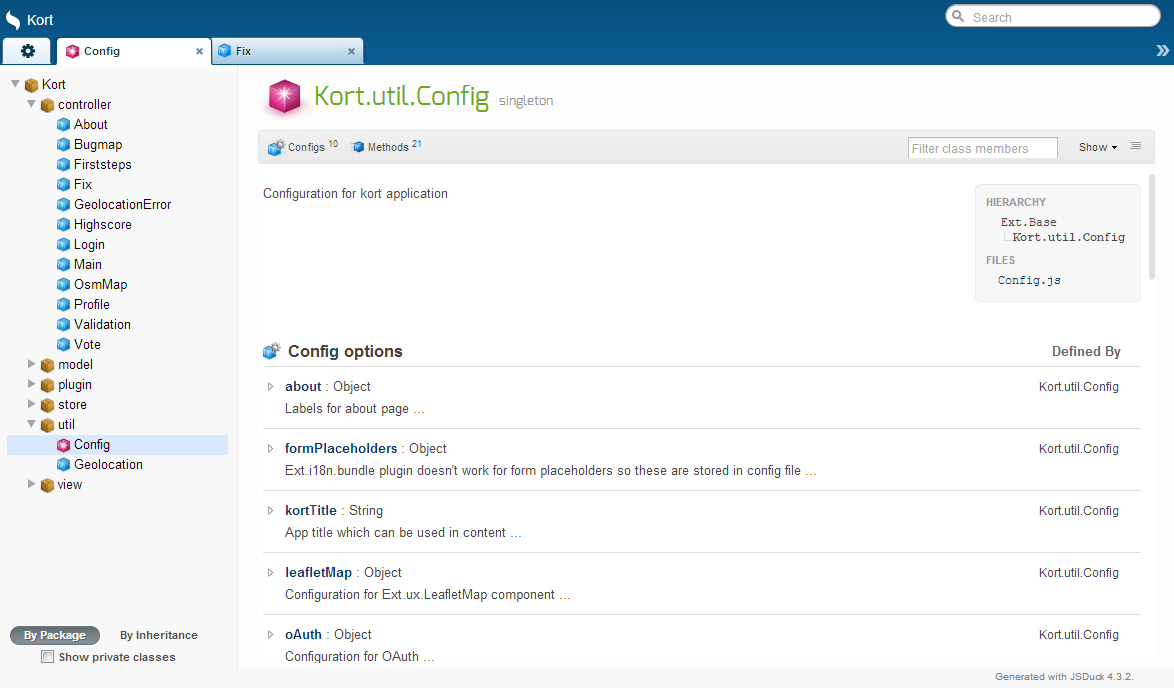
\includegraphics[scale=0.33]{images/implementation/frontend/kort-documentation}
	\caption{Frontend Dokumentation mit JSDuck}
	\label{image-kort-documentation}
\end{figure}

% Bekannte Fehler
% Bekannte Fehler
\section{Bekannte Fehler}

\subsection{iOS6 - Add to homescreen}
Eine sehr nützliche Funktionalität, welche Apple im Mobile Safari-Browser anbietet ist die \emph{Add to homescreen}-Funktion.

\begin{figure}[H]
\subfigure{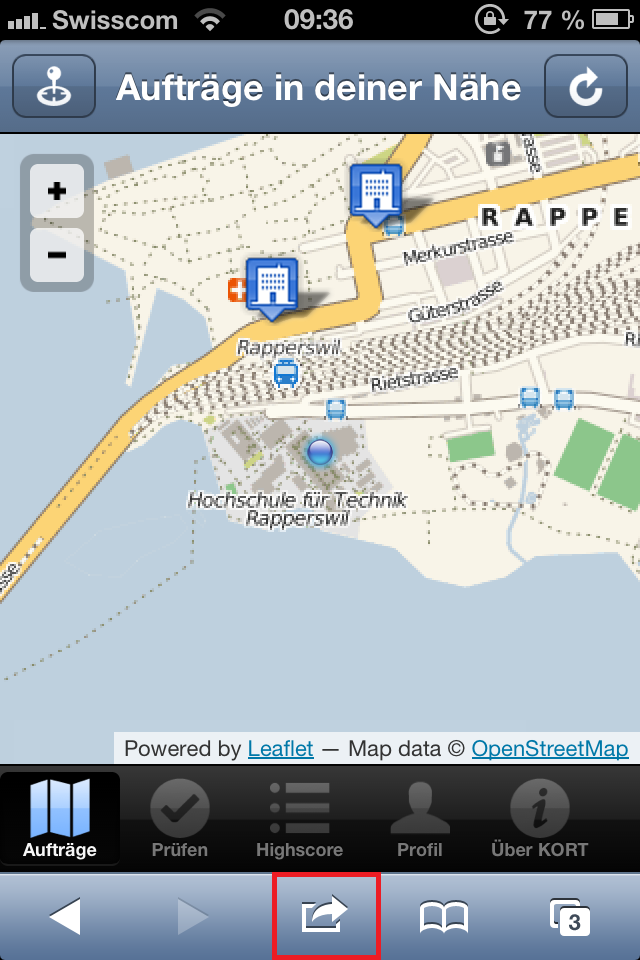
\includegraphics[width=0.23\textwidth]{images/bugs/kort-add_to_homescreen_1}}
\hfill
\subfigure{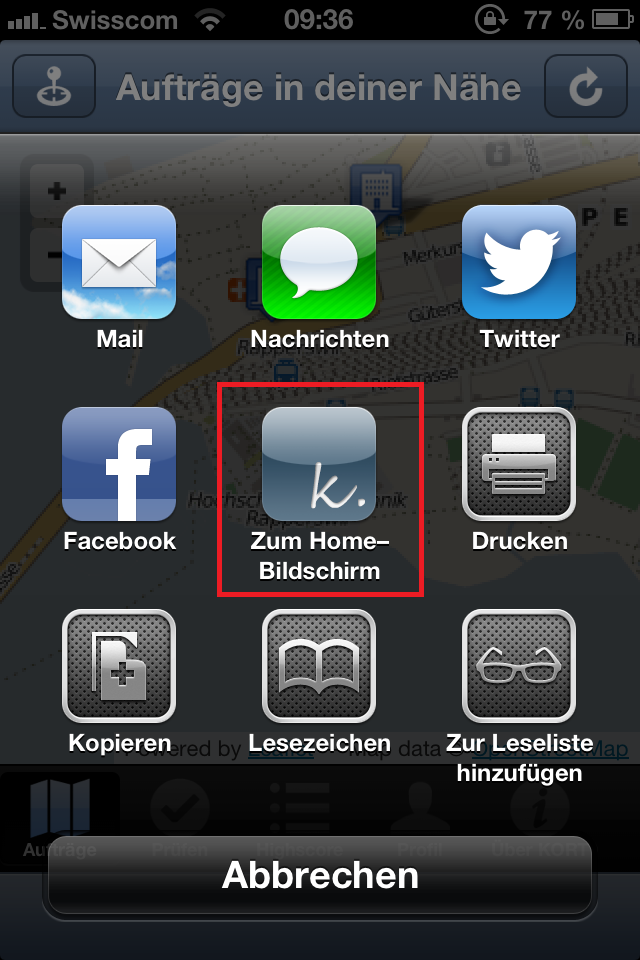
\includegraphics[width=0.23\textwidth]{images/bugs/kort-add_to_homescreen_2}}
\hfill
\subfigure{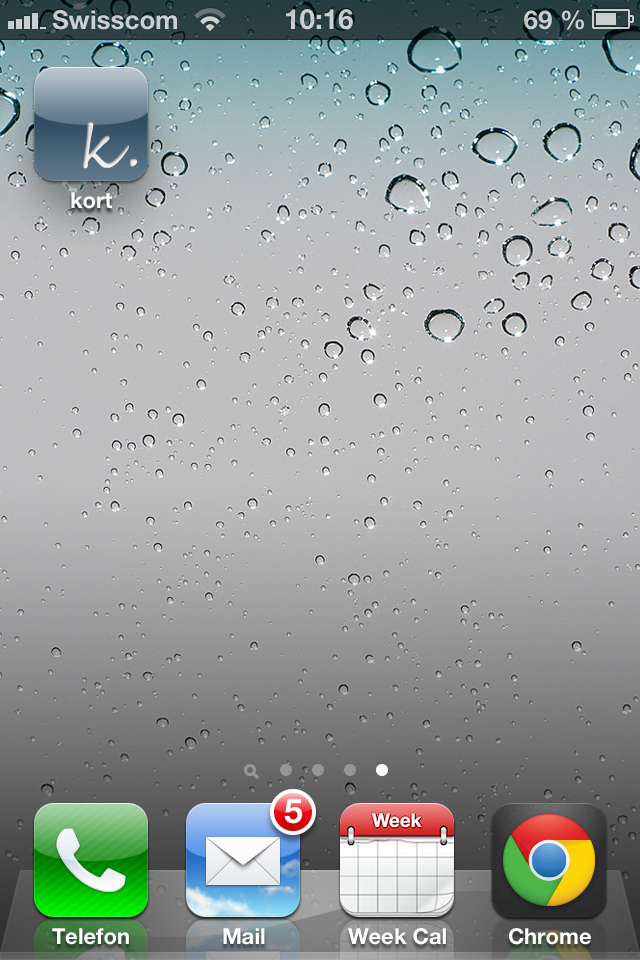
\includegraphics[width=0.23\textwidth]{images/bugs/kort-add_to_homescreen_3}}
\hfill
\subfigure{
\includegraphics[width=0.23\textwidth]{images/bugs/kort-add_to_homescreen_4}}
\caption{iOS Add to homescreen-Funktion}
\end{figure}

Dadurch wird ein App-ähnliches Bookmark der aktuellen Webseite auf dem Homescreen erstellt.
Dieser erhält ein hinterlegtes Icon und einen Titel.
Beim Starten der App erscheint ein Splashscreen, welchen man ebenfalls in der Webseite definieren kann.
Zudem öffnet sich der Browser ohne jegliche Toolbars wie  Adress- oder Navigationsleiste.

Leider befindet sich in iOS6 ein Bug, welcher den Zugriff auf die Geolocation verhindert, wenn die \gls{WebApp} vom Homescreen aus gestartet wird.
Auf StackOverflow\footnote{\url{http://stackoverflow.com/questions/12503815/ios-6-breaks-geolocation-in-webapps-apple-mobile-web-app-capable}} wird der Bug genauer beschrieben.

\subsubsection{Workaround}
Im Sencha Forum\footnote{\url{http://www.sencha.com/forum/showthread.php?246317-2.1.0-RC1-Save-to-home-screen-Geolocation-not-working}} wird als Workaround vorgeschlagen, die Generierung des \newline \inlinecode{apple-mobile-web-app-capable} Metatags in der Sencha Touch Library zu deaktivieren (siehe Code-Ausschnitte \ref{code-ios6-homescreen-metatag} und \ref{code-ios6-bug-workaround}).

\lstset{language=HTML}
\begin{lstlisting}[caption=Metatag{,} welcher iOS6 Bug hervorruft, label=code-ios6-homescreen-metatag]
<meta content="yes" name="apple-mobile-web-app-capable" />
\end{lstlisting}

\lstset{language=JavaScript}
\begin{lstlisting}[caption=iOS6 Bug Workaround, label=code-ios6-bug-workaround]
//meta('apple-mobile-web-app-capable', 'yes');
\end{lstlisting}

Das Deaktivieren dieser Zeile hat aber zur Folge, dass der native Rahmen des Browsers (Adressleiste, Navigationsleiste) wieder angezeigt wird.
Dies ist zwar unschön, löst aber das Problem mit dem Zugriff auf die Geolocation.

\subsection{App Build}
Wie in Abschnitt \ref{sencha-cmd} beschrieben, basiert die App vollständig auf dem Sencha-eigenen Build-Tool \brand{Sencha Cmd}. Darin sind aber noch einige Bugs vorhanden.

Bei \kort{} besteht dabei ein Problem bei der fest eingebauten Komprimierung der JavaScript-Sourcen.
Während diesem Prozess werden lokale Variablennamen mit einzelnen Buchstaben abgekürzt, um die Dateigrösse zu reduzieren.
Dabei treten Konflikte mit der \brand{Leaflet}-Library auf, welche den Buchstaben \emph{L} als Namespace verwendet.

\subsubsection{Workaround}
Um diese Problem zu umgehen, mussten wir das Build-Skript von \brand{Sencha Cmd} minimal anpassen.
So mussten wir die Zeile, welche den \gls{Microloader} komprimiert, auskommentieren (siehe Code-Ausschnitt \ref{senchacmd-workaround}).
Diese befindet sich in folgender Datei:

\inlinecode{/<Sencha Cmd Verzeichnis>/plugins/touch/current/app-build.js} Zeile 362

\lstset{language=JavaScript}
\begin{lstlisting}[caption=Sencha Cmd Workaround, label=senchacmd-workaround]
processIndex = function () {
	[...]
	compressor = new ClosureCompressor();
	microloader = (environment == 'production'
		? 'production'
		: 'testing') +
		'.js';
	_logger.debug("using microloader : {}", microloader);
	content = readFileContent(joinPath(sdk, "microloader", microloader));
	//content = compressor.compress(content);
	remotes = [
		'<script type="text/javascript">' +
			content + ';Ext.blink(' +
			(environment == 'production' ? jsonEncode({
				id:config.id
			}) : appJson) + ')' +
			'</script>'
	];
	[...]
};
\end{lstlisting}